%!TEX root = ../../main.tex
\section{Interface}
Interfacet (\gls{gui}'en) kan tilgås via en webbrowser som med udgangspunkt ligner Figur \ref{fig:index} og \ref{fig:kar}.
\begin{figure}[H]
    \centering
    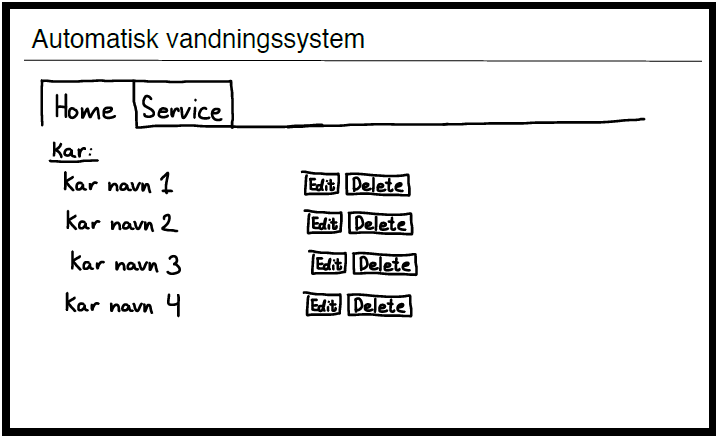
\includegraphics[width=0.7\textwidth]{Kravspecifikation/Interface/photo/index.PNG}
    \caption{AVS Interface - home}
    \label{fig:index}
\end{figure}
På Figur \ref{fig:index} kan brugeren se en liste over de kar der er oprettet, hvor de forskellige kar kan tilgås hvis brugeren klikker på det ønskede kar. 
\\\\
Under service har teknikeren mulighed for at oprette et \gls{kar}, hvor han indtaster adresse, navn og derefter trykker opret \gls{kar}. hvorefter karet kommer frem på listen over \gls{kar}. ydermere er der en delete og edit knap uden for hvert \gls{kar} så teknikeren har mulighed for at slette et \gls{kar} eller redigerer navnet. 
\\\\
Når brugeren trykker på et \gls{kar} tilgår han/hun et interface for \gls{kar}et, som kan ses på Figur \ref{fig:kar}. 
\begin{figure}[H]
    \centering
    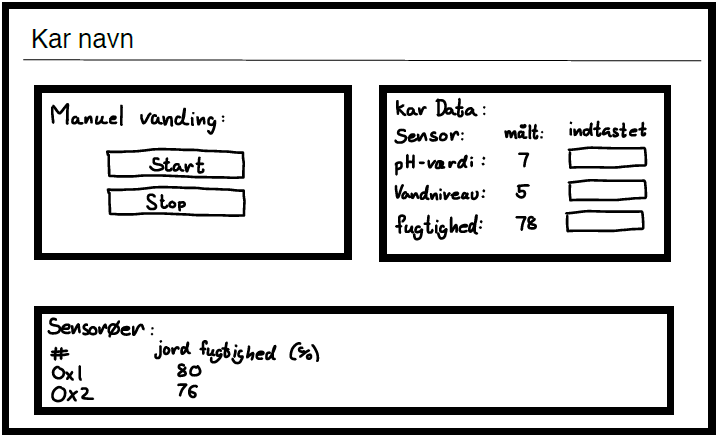
\includegraphics[width=0.7\textwidth]{Kravspecifikation/Interface/photo/kar.PNG}
    \caption{AVS Interface - kar}
    \label{fig:kar}
\end{figure}

I feltet øverste til venstre er der mulighed for manuel vanding, hvor brugeren trykker på start når han/hun vil starte den manuelle vanding. For at stoppe den manuelle vanding trykke på bruger på stop.   
\\\\
I feltet øverst til højre har brugeren mulighed for at indtaste de ønskede data og aflæse de data der kommer fra de forskellige sensor. 
\\\\
I det nederste felt kan der ses en liste over \gls{sensoroe}erne hvor brugeren kan aflæse de data der kommer fra de forskellige sensor.   